% Author: David Sanchez-Jacome

\chapter{Fundamentals of Programmable Integrated Photonics} \label{chap:fundamentals}

The evolution of integrated photonics has led to the development of programmable photonic circuits, enabling flexible and reconfigurable optical signal processing.
Unlike fixed-function photonic circuits, programmable architectures provide the ability to dynamically adapt their functionality.
This chapter explores the fundamental components that form the foundation of programmable integrated photonics.
We begin by examining the building blocks of these circuits, including optical waveguides, phase shifters, and couplers, which serve as the core elements for light manipulation.
Next, we delve into recirculating photonic meshes, the scalable architectures that enable complex optical transformations through interconnected tunable elements.
Following this, we introduce iPronics first-generation Smartlight solution, a leading implementation of general-purpose programmable photonics, demonstrating the transition from academic research to real-world applications.
Finally, we discuss the software stack that enables seamless control of these photonic processors, bridging the gap between hardware and high-level applications.

\section{Building blocks} \label{sec:building_blocks} % (fold)
\subsection{Optical waveguides} \label{sub:optical_wg} % (fold)

\begin{figure}[h]
	\begin{center}
		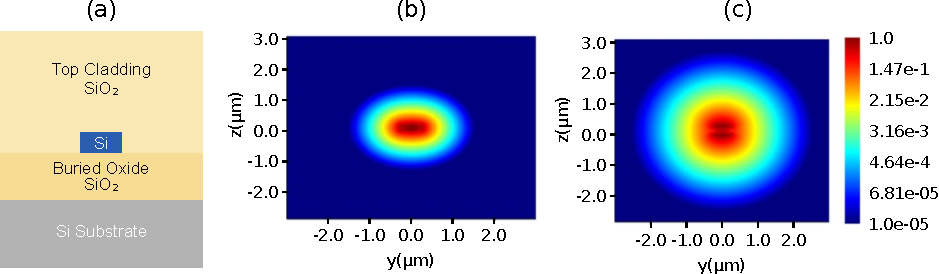
\includegraphics{figures/ch2-wg.pdf}
	\end{center}
	\caption{Optical strip waveguide. (a) Material cross-section showing the high-index \ce{Si} core surrounded by the \ce{SiO2} cladding. (b) and (c) show the first TE and TM propagation mode's field
		intensity, respectively.}\label{fig:ch2-wg}
\end{figure}

Integrated optical waveguides are the foundational components of photonic integrated circuits (PICs), enabling the propagation of optical signals within a confined medium.
Structurally, waveguides function as optical counterparts to electrical transmission lines, utilizing total internal reflection (TIR) to guide light through a high-refractive-index core surrounded by a lower-refractive-index cladding.
The most prevalent waveguide configurations include strip waveguides, which are fully etched channels embedded in a planar substrate, and rib waveguides, which feature a partially etched ridge atop a lower-index slab, providing enhanced modal confinement and reduced propagation losses.
These structures can be fabricated from a variety of materials, including silicon \cite{siew_review_2021}, silicon nitride \cite{xiang_silicon_2022}, indium phosphide \cite{smit_past_2019} and lithium niobate \cite{boes_lithium_2023}, each offering distinct advantages in terms of propagation loss, nonlinearity, and compatibility with complementary metal-oxide-semiconductor (CMOS) processes.
One of the main key issues addressed by fabrication foundries is insertion losses (IL) of the waveguides.
The minimization of this parameter from a couple of \(dB/cm\) to \(dB/m\) is crucial in enabling large-scale photonic integration.
This, in turn, will make possible the that integrated applications can compete directly with existing free-space solutions.

Integrated waveguides serve a critical role in modern photonic systems, facilitating functionalities such as optical signal routing, modulation, switching, and multiplexing.
Through different design geometries they can take the form of devices like Mach-Zehnder interferometers (MZIs), micro ring resonators (MRRs), delay lines (DLs), among many others.
Figure~\ref{fig:ch2-wg} depicts the cross-section of an optical waveguide used in the first-generation Smartlight platform (a).
This waveguide has a width of 0.5~um and a height of 0.22~um and a typical loss of 2.5~\(dB/cm\) in the C-band \cite{perez-lopez_general-purpose_2024}.
Next to it in (b) and (c) we observe the simulated field distribution for the first TE and TM modes respectively.
For further theory related to light confinement in semiconductor waveguides refer to \cite{chrostowski_silicon_2015,saleh_guided-wave_1991}.
% subsection Optical waveguides (end)

\subsection{Splitters}\label{sub:splitters} % (fold)

\begin{figure}[h]
	\begin{center}
		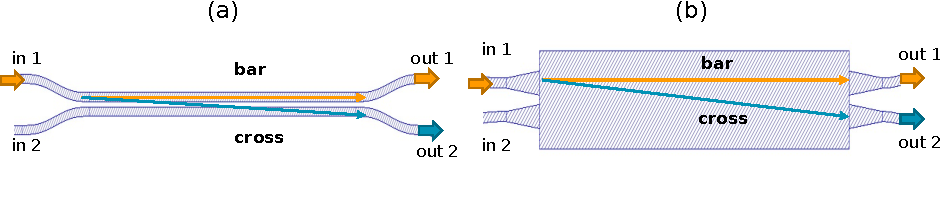
\includegraphics{figures/ch2-splitters.pdf}
	\end{center}
	\caption{Schematic representation of a directional coupler (DC) (a) and a multimode interferometer (MMI) (b) used to split optical signals.}\label{fig:ch2-splitters}
\end{figure}

Optical splitters are passive photonic devices that divide or combine optical signals in integrated photonic circuits.
They are fundamental building block to perform to efficient and low-loss signal distribution and routing.
In integrated photonics, two of the most commonly used optical splitters are Directional Couplers (DCs) and Multimode Interferometers (MMIs).

Directional Couplers (DCs) are passive components that use evanescent coupling between two adjacent waveguides to perform the splitting operation.
When these two optical waveguides are placed close together (typically a few hundred nm) their evanescent fields overlap, allowing light to tunnel from one waveguide to the other.
This phenomenon, known as evanescent coupling, is the fundamental mechanism behind directional couplers \cite{tormen_wavelength-flattened_2005,chen_broadband_2017,chen_low-loss_2016}.
Because of this, DCs are highly dependent on wavelength, waveguide separation, and coupling length.
Similarly, the dependence on very small waveguide gaps makes them sensitive to small variations in waveguide fabrication.
In terms of footprint, they are typically longer than MMIs as they are restricted by the coupling length.
One advantage over MMIs is that they can be tuned dynamically via phase shifters to control its output phase and amplitude response \cite{perez-lopez_integrated_2019}.
DCs usually yield lower insertion loss (\(IL = [0.1, 0.5]\) dB) but are susceptible to coupling imbalances due to fabrication tolerances \cite{darmawan_rigorous_2005}.

A Multimode Interferometer (MMI) is a passive photonic device used for splitting, combining, and routing optical signals in integrated photonic circuits.
It operates based on self-imaging in multimode waveguides, where an input optical field forms multiple replicas at specific distances inside the waveguide due to interference between supported modes.
When light enters the multimode waveguide, it excites multiple propagation modes.
These modes interfere constructively and destructively at different points, forming periodic self-images.
Depending on the length and width of the MMI, different power-splitting ratios can be achieved \cite{soldano_optical_1995,sheng_compact_2012}.
Mathematically, the self-imaging effect in an MMI is determined by its length \( L \) and effective refractive index \( n_{\text{eff}} \), which define the position of constructive interference patterns.
These components can perform a large variety of splitting ratios (1×2, 1×N, N×M configurations) to distribute signals efficiently \cite{hosseini_1_2011}.
Unlike directional couplers, MMIs are less sensitive to fabrication variations, ensuring high yield and reliability in large-scale photonic chips.
If designed correctly these components can also occupy a small footprint which favors large-scale integration \cite{kim_experimental_2022}.
Even though MMIs introduce higher insertion losses than directional couplers (\(IL = [0.2, 0.8]\) dB), their high yield and fabrication tolerance makes them a very attractive solution for large integrated distribution circuits \cite{darmawan_rigorous_2005}.
Because of these reasons MMIs are widely used as power splitters, combiners, and switches in PICs \cite{song_low-loss_2022}.

Figure~\ref{fig:ch2-splitters} shows the schematics of both a DC (a) and an MMI (b) from one of the several chips fabricated by iPronics in the time frame of this thesis.
These components have been optimized to achieve as low-loss and small footprint as possible to favor high-density integration in our chips.
The splitter chosen for our main designs is the MMI as it provides the low-loss, fabrication tolerance and broadband specs required by the applications that will be presented in Chapter~\ref{chap:applications_using_fppgas}.

Several MMI/DC designs are simulated, sent for tape-out and characterized in our lab facilities before they are included as part of our final chips.
Typically, once the best components have been filtered out during the simulation stage, they are included in test dies that are fabbed in multiproject wafer (MPW) runs.
Once the chips, reach our facilities they are characterized in terms of insertion losses, crosstalk and reflection in order to select the best candidates that will be included in our main mesh circuits.

% subsection Splitters (end)

\subsection{Phase shifters}\label{sub:phase_shifters} % (fold)

\begin{figure}[h]
	\begin{center}
		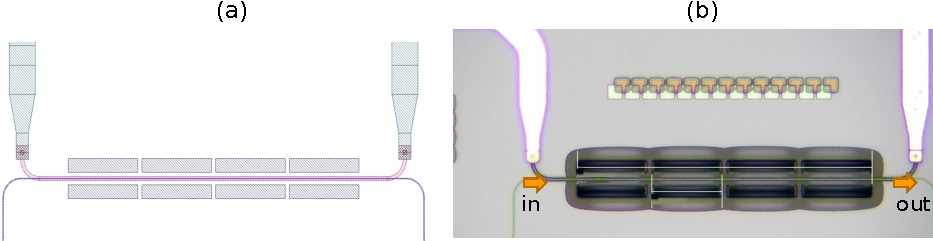
\includegraphics{figures/ch2-phase_shifter.pdf}
	\end{center}
	\caption{(a) Schematic representation and (b) microscope picture of a thermo-optic phase shifter fabricated to provide reconfigurability to the underlying PIC structure.}\label{fig:ch2-phase_shifter}
\end{figure}

A phase shifter is a key component in programmable integrated photonics.
It's responsible for modulating the phase of an optical signal as it propagates through a waveguide.
By controlling the phase of light, phase shifters enable essential functions such as beam steering, optical interference control, and signal processing in photonic circuits.
A phase shifter modifies the optical path length of a waveguide by altering its refractive index or physical length.
The phase of a light wave traveling through a waveguide is defined by:

\begin{equation}
	\phi = \frac{2\pi n_{eff}
		L}{\lambda} \label{eq:ch1-phase_shift} \end{equation}

where \( n_{eff} \) is the effective refractive index, \( L \) is the waveguide length, and \( \lambda \) is the optical wavelength in vacuum.
Changing either \( n \) or \( L \) causes a shift in the optical phase \cite{chrostowski_silicon_2015}.

There are different types of phase shifters in photonic integrated circuits:

\begin{itemize}
	\item Thermo-Optic Phase Shifters (TOPS): Based on heating a waveguide to change its refractive index.
	      They are comparably slow (µs response time), but low power and widely used in silicon photonics.
	      Commonly found in Mach-Zehnder interferometers (MZIs) and programmable photonic meshes \cite{jacques_optimization_2019, liu_thermo-optic_2022}.
	\item Electro-optic Phase Shifters: Make use of an electric field to change the refractive index through the Pockels effect.
	      Found in materials like lithium niobate (\ce{LiNbO3}) or III-V semiconductors.
	      They are much faster (ps–ns range) than thermo-optic phase shifters, making them ideal for high-speed modulators \cite{maldonado_electro-optic_1995,yoshioka_cmos-compatible_2024}.
	\item Carrier Injection/Depletion Phase Shifters: Based on using free carrier-flow (electrons/holes) to modify the refractive index.
	      Implemented in silicon photonics via PN-junctions or MOS capacitors.
	      Faster than thermo-optic phase shifters (ns range) but more lossy \cite{gabriel_performance_2020,kruckel_towards_2021}.
	\item MEMs-Based Phase Shifters: Use micro-electromechanical actuators to change the waveguide position or structure.
	      Extremely low power consumption but require high voltages and their process nodes have lower maturity/reliability.
	      Useful in tunable optical circuits and programmable photonic chips \cite{errando-herranz_mems_2020,quack_integrated_2023}.
\end{itemize}

Phase shifters are essential for dynamically controlling light in reconfigurable photonic circuits.
In the last decade they have enabled the demonstration of large array reconfigurable PICs.
These applications span the fields of optical switching for datacenter networking, beam steering phased array antennas, quantum photonics and photonic neural networks.

Figure~\ref{fig:ch2-phase_shifter} shows the schematic (a) and microscope photography (b) of a thermo-optic phase shifter deployed in the framework of this thesis.
The actuators use under-etch technology to provide thermal isolation to mitigate thermal crosstalk and provide higher rise time.
As observed in the figure, trenches have been placed next to the high resistance heating material to create air isolation around it and the underlying waveguide.
To better understand thermal crosstalk and how this design mitigates it refer to Section~\ref{sec:thermal_crosstalk}.

% subsection Phase shifters (end)
\subsection{The Mach-Zehnder interferometer}\label{sub:the_mach-zehnder-interferometer} % (fold)

\begin{figure}[h]
	\begin{center}
		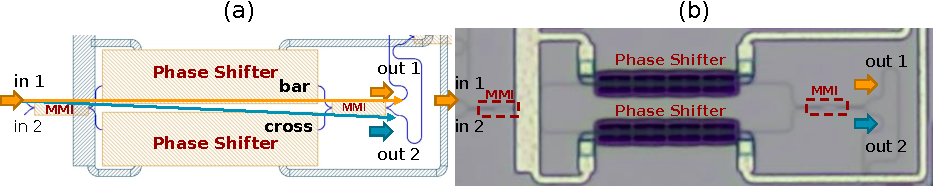
\includegraphics{figures/ch2-mzi.pdf}
	\end{center}
	\caption{Schematic representation (a) and microscope photography (b) of the fabricated MZIs.
		The chosen design uses MMIs are optical splitters and two underetched phase shifter to provide accurate control of phase and amplitude at the interferometer's output.
	}\label{fig:ch2-mzi}
\end{figure}

A Mach-Zehnder interferometer (MZI) is an optical device that splits and recombines light waves to create interference patterns.
The MZI operates by splitting an input light wave into two paths, modulating them separately, and then recombining them to analyze interference effects.
This allows precise monitoring of phase, amplitude, and wavelength of light \cite{mach_ueber_1892,zehnder_neuer_1891}.
Because of this, it is widely used in optical communication, sensing, metrology, and programmable photonics.

In free-space optics, a traditional Mach-Zehnder Interferometer consists of two beam splitters and two mirrors that create two distinct optical paths.
A coherent light source enters the first beam splitter, which divides the light into two separate beams traveling along different arms of the interferometer.
Each beam travels through its own optical path, which can include phase modulators, delay elements, or medium variations that affect the phase difference between them.
The two beams meet at a second beam splitter, where they interfere constructively or destructively depending on their phase difference.
The resulting interference pattern is measured at the output ports, providing information about path differences, refractive index changes, or external modulations \cite{saleh_wave_1991}.
Free-space MZIs are widely used in interferometric sensing, optical coherence tomography (OCT), and precision metrology, where detecting small phase shifts is critical \cite{hariharan_interferometry_2005,fujimoto_optical_2003}.

In integrated photonics, the free-space optics components (beam splitters, mirrors, and modulators) are replaced by on-chip waveguides and phase shifters.
Instead of bulk beam splitters, MMIs or DCs divide the light into two waveguide arms.
The waveguides include thermo-optic, electro-optic, or carrier-injection phase shifters, allowing dynamic phase control.
After phase modulation in the arms, the light recombines at a second waveguide splitter, producing an interference pattern that can be either detected electronically or used for further optical processing.
The advantage of integrated MZIs is that they enable high-density integration for large-scale photonic circuits, allowing for real-time reconfiguration and high-speed processing in applications like optical switching, modulators, LiDAR, quantum photonics and photonic neural networks \cite{capmany_programmable_2020}.
The concept of programmable integrated photonics (PIP) is driven by this motivation to integrate high MZI counts, and other tunable elements, to favor the development of novel photonic solutions.

Figure~\ref{fig:ch2-mzi} depicts the schematic (a) and a microscope photography (b) of one of the MZIs in the first-generation Smartlight processor.
Notice that it's composed by two MMIs (input/output) and two thermo-optic phase shifters (one per arm).
The circuit is balanced as both arms have the same length.
The two actuators allow control over the phase and amplitude response of the circuit.
From now on in this document we will refer to this type of MZI, a balanced dual-driven one, as a \textbf{programmable unit cell (PUC)} to emphasize its role as the basic reconfigurable building block for this thesis.
The transfer matrix representing a PUC for a fixed state of polarization and lossless propagation is given by Equation~\eqref{eq:ch2-puc}

\begin{equation}
	\label{eq:ch2-puc}
	\begin{aligned}
		T_{PUC} & =
		\begin{bmatrix} \sqrt{\rho} & j\sqrt{1-\rho} \\ j\sqrt{1-\rho} & \sqrt{\rho} \end{bmatrix}
		\cdot
		\begin{bmatrix} e^{j\phi_{up}} & 0 \\ 0 & \phi_{lo} \end{bmatrix}
		\cdot
		\begin{bmatrix} \sqrt{\rho} & j\sqrt{1-\rho} \\ j\sqrt{1-\rho} & \sqrt{\rho} \end{bmatrix} \\
		        & =
		je^{j\Delta}
		\begin{bmatrix}
			sin(\theta) & cos(\theta)  \\
			cos(\theta) & -sin(\theta)
		\end{bmatrix}.
	\end{aligned}
\end{equation}
where \(\phi_{up},\) and \(\phi_{lo}\) correspond to the upper and lower driving phases.
$\Delta = (\phi_{up} + \phi_{lo})/2$ is what we will refer from on as the \textbf{cross-phase}, and it's a measure of the common phase at the PUC's outputs.
$\theta = (\phi_{up} - \phi_{lo})/2$ is related to the \textbf{coupling factor \(k\)} through the \(k = cos(\theta)\) relationship.
The coupling factor is a critical metric because it defines the amplitude response of the PUC at each output.
\(\rho\) is the MMI's power splitting ratio and is considered to be 0.5 for an ideal 3-dB coupler \cite{shokraneh_theoretical_2020}.
The experimental measurement of the PUC's transfer matrix will be covered in detail later in this chapter alongside Figure~\ref{fig:ch2-sw-calib}.

\subsection{Integrated photonic resonant devices}\label{sub:integrated_photonic_resonant_devices} % (fold)
\begin{figure}
	\begin{center}
		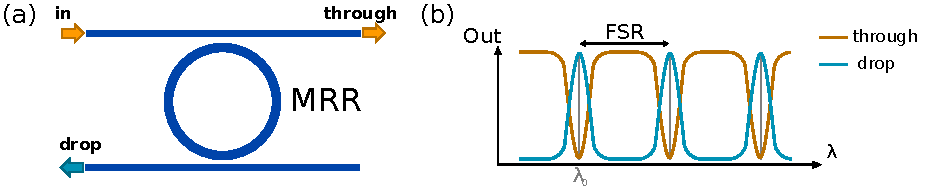
\includegraphics{figures/ch2-ring.pdf}
	\end{center}
	\caption{Basic configuration (a) of a MRR in PIC circuits.(b) Shows the optical response on the through and drop ports}\label{fig:ch2-ring}
\end{figure}

Resonant devices are key components in PICs and are designed to selectively interact with light at specific wavelengths through the principle of resonance.
They achieve this by trapping and intensifying light within an optical cavity at particular resonant wavelengths.
They are characterized by their resonant wavelength, Free Spectral Range (FSR), and Quality Factor (Q-factor).
A high Q-factor signifies a sharp, narrow resonance and excellent energy storage, crucial for applications demanding high spectral selectivity or sensitivity \cite{bogaerts_silicon_2012}.

Microring resonators (MRRs) are the most common resonant structure in silicon photonics PICs.
An MRR is essentially a waveguide formed into a closed loop, where light couples in from an adjacent "bus" waveguide via evanescent waves.
Resonance occurs when the optical path length around the ring is an integer multiple of the ring's resonant wavelength, leading to constructive interference.
When light is "on-resonance," it efficiently couples into the ring, building up intensity and appearing at a "drop" port (in an add-drop configuration) or causing a dip in the "through" port (in an all-pass configuration).
Light that's "off-resonance" passes through with minimal interaction \cite{chao_polymer_2006}.

MRRs offer several advantages: they are compact, allowing for high integration density, and can achieve very high Q-factors, leading to precise spectral filtering.
They are also highly versatile, functioning as filters, modulators, switches, and sensors.
Their resonant wavelength can be tuned using various effects, such as thermo-optic or electro-optic changes \cite{bawankar_microring_2021}.
However, MRRs do come with challenges \cite{little_toward_2000}.
Their performance is highly sensitive to fabrication variations, meaning tiny manufacturing imperfections can significantly alter their resonant properties.
They are also susceptible to temperature fluctuations due to the thermo-optic effect, often requiring active thermal stabilization.
Overcoming these challenges is a major focus in current PIC research and development.

% subsection Integrated photonic resonant devices (end)
% subsection The Mach-Zehnder interferometer (end)
\section{Recirculating Meshes}\label{sec:recirculating_meshes} % (fold)

\begin{figure}[h]
	\begin{center}
		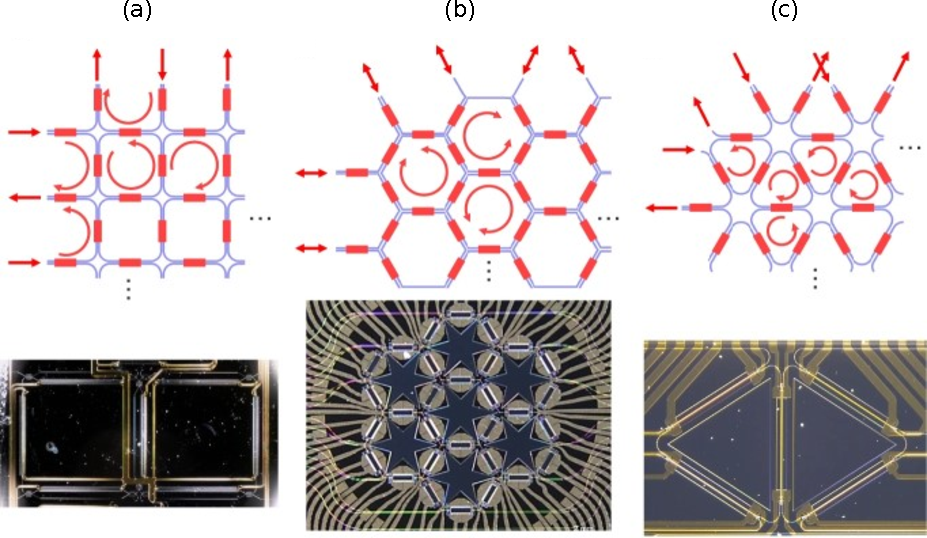
\includegraphics{figures/ch2-recirculating.pdf}
	\end{center}
	\caption{Schematic representation (top) and microscope photography (bottom) of square, hexagonal and triangular based recirculating meshes.
		Photographs reproduced from \cite{zhuang_programmable_2015}, OSA Publishing (a), \cite{perez_multipurpose_2017}, Springer Nature (b) and \cite{perez-lopez_integrated_2019}, OSA Publishing (c).
		Schematics reproduced from \cite{bogaerts_programmable_2020}, Springer Nature.
	}\label{fig:ch2-recirculating}
\end{figure}

Recirculating meshes consist of an array of PUCs coupled together using optical waveguides to create a regular a two-dimensional (2D) grid of loops.
These photonic circuit architectures incorporate feedback loops to enable complex optical transfer functions.
Unlike feedforward meshes, which rely solely on cascading interferometers, recirculating meshes introduce multi-path interference and resonant effects, providing additional functionality in filtering, delay engineering, and signal processing.
A key advantage of recirculating meshes is their ability to implement higher-order spectral filtering, making them useful in applications requiring precise wavelength selection as shown in Section~\ref{sec:filters}.
Additionally, they allow for programmable dispersion and optical delay, enabling advanced signal-processing functionalities such as optical buffering and equalization (refer to Sec~\ref{sec:reconfigurable_delay_lines}).
Their compact nature also offers benefits in circuit integration, as they provide complex operations without requiring long cascades of optical elements.
These meshes can also be programmed as forward-only arrays (although using more PUCs) as will be discussed in detail in Chapter~\ref{chap:universal_unitary_operators}.

Figure~\ref{fig:ch2-recirculating} showcases different recirculating photonic mesh architectures used in programmable photonic circuits.
It consists of square \cite{zhuang_programmable_2015}, hexagonal \cite{perez_multipurpose_2017} and triangular \cite{perez-lopez_integrated_2019} architectures (a, b, and c, respectively).
The top row presents schematic representations of the photonic meshes, where red elements correspond to PUCs, and blue lines represent optical waveguides.
The arrows illustrate the input and output ports, as well as the propagation directions of light within the structures.
The bottom row contains microscope images of the corresponding fabricated photonic chips.
When comparing these topologies \cite{perez_reconfigurable_2016-1,capmany_programmable_2020} against each other using metrics such as PUCs per area, reconfigurability, and filter periodicity (among others), the hexagonal mesh comes on top, especially because all ports can function as inputs/outputs (I/O) \cite{bogaerts_programmable_2020}.

Due to the integration complexity, these architectures introduce significant control and stability challenges.
The presence of feedback loops demands precise pre-characterization or optimization methods to prevent unwanted resonances or instability \cite{perez-lopez_multipurpose_2020,perez-lopez_programmable_2020}.
Moreover, optical losses accumulate with each round trip inside the loop, which can degrade overall performance.
In silicon photonics, where propagation losses are non-negligible, this poses a major design constraint.

Despite these challenges, recirculating meshes have found applications in programmable optical filters, optical delay lines, and reconfigurable photonic processors.
Their ability to manipulate optical signals dynamically makes them particularly valuable in telecommunications, signal processing, and even quantum photonics.
Chapter~\ref{chap:applications_using_fppgas} covers in detail the advanced programming strategies required to implement and experimentally validate several applications in the hexagonal mesh developed by iPronics for its first-generation Smartlight platform.

\section{Smartlight: The Field Programmable Photonic Gate Array}\label{sec:smartlight_fppga}

\begin{figure}[h]
	\begin{center}
		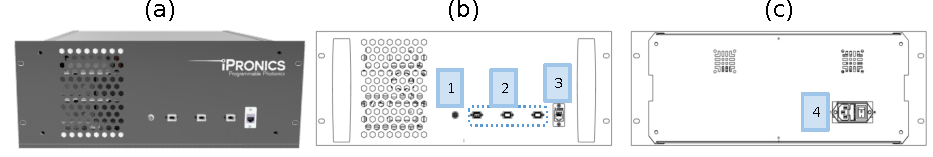
\includegraphics{figures/ch2-smartlight.pdf}
	\end{center}
	\caption{Photography of a first-generation Smartlight processor (a) and schematics of its front (b) and back panels (c).
		External interfaces are numbered: (1) Laser output, (2) Optical ports (3 MTP/MPO connectors, 72 optical ports), (3) Ethernet communication port, (4) Power supply input.
	}\label{fig:ch2-smartlight}
\end{figure}

The general-purpose photonic processor presented in this work aggregates, for the first time, the complex full-stack necessary to operate a programmable photonic device: the optical layer, the control layer, and the software layer.
The processor has been named, and will be referred hereafter, as the iPronics Smartlight Processor.
The first-generation Smartlight is contained in a 4U rack box with two front handles as shown in Figure~\ref{fig:ch2-smartlight}(a).
Fig.~\ref{fig:ch2-smartlight} (b) depicts the front panel which contains, from left to right, a ventilation hexagonal grid, a laser optical output through an FC/APC optical connector (1), three MTP optical connectors with 24 channels each (2), and a Cat-6 Ethernet female connector (3), which is physically connected to the control unit of the iPronics Smartlight processor.
The back panel, shown in Fig.~\ref{fig:ch2-smartlight}(c) contains the main power socket IEC C14 (4) located on the right side, together with an ON-OFF switch.
Also, in the upper part there are two ventilation grills holding two air fans in the inside.

\subsection{General specifications}\label{sub:general_specifications} % (fold)

The general specifications of the first-generation Smartlight system are presented in Table~\ref{tab:ch2-gen-specs} where most of the externals provisions are detailed.
Notably, the units come equipped with an internal tunable laser source to enable standalone operation without any third-party equipment.
The system consumes less than 20 W and has been designed and engineered to work in the C-band for telecom applications.

% \begin{noindent}
\begin{table}[h!]
  \small
	\centering
	\begin{tabular}{|m{4cm}|m{1.0cm}|m{1.0cm}|m{1.0cm}|m{1.5cm}|m{5.5cm}|}
		\hline
		\multirow{2}{*}{\textbf{Specification}} & \multicolumn{3}{c|}{\textbf{Value}} & \multirow{2}{*}{\textbf{Units}} & \multirow{2}{*}{\textbf{Description}}                                                                                                                                                 \\
		\cline{2-4}  % Line only below column 2 
		                                        & Min                                 & Typ.                            & Max                                   &           &                                                                                                                                   \\
		\hline
		Number of optical channels              &                                     & 28                              &                                       &           & The optical ports are connected to the PIC through 3 MTP/MPO connectors located on the front panel.
		\\
		\hline
		Number of laser optical outputs         &                                     & 1                               &                                       & output    & There is one laser output FC/APC located on the front panel that can be controlled by software.
		\\
		\hline
		Power supply                            &                                     & 1                               &                                       & port      & An IEC13 connector feeds the power supply (230V/110V) of the photonic processor.
		\\
		\hline
		Dimensions                              &                                     & 425 \times 425 \times 173       &                                       & mm$^3$    & The chassis is compatible with
    standard 19" rack sizes.                                                                          \\
		\hline
		Communication ports                     &                                     & 1                               &                                       & ports     & A BLE Gigabit Ethernet connector enables communication with the logic unit of the photonic processor.
		\\
		\hline
		Power consumption                       &                                     & $<$20                           &                                       & W         & Total power consumption is less than 20 W.
		The photonic IC consumes less than 1 W.
		\\
		\hline
		Weight                                  &                                     & $<$12                           &                                       & Kg        &                                                                                                                                   \\
		\hline
		Wavelength range of operation           & 1520                                & 1530-1580                       & 1600                                  & nm        & The device is designed to work
    at \textbf{1550 nm} for TE polarization over a 100 nm bandwidth.
		\\
		\hline
		Laser power range                       & -1                                  & 9                               & 10                                    & dBm       &                                                                                                                                   \\
		\hline
		Laser wavelength                        &                                     & 1549.5-1552                     &                                       & nm        &                                                                                                                                   \\
		\hline
		Laser frequency adjust                  &                                     & $\pm$0.24                       &                                       & nm        &                                                                                                                                   \\
		\hline
		Operating temperature (external)        & 0                                   & 5–55                          & 65                                    & $^\circ$C & Ambient temperature range supported by the system.                                                                                \\
		\hline
	\end{tabular}
	\caption{General specifications of a first-generation Smartlight unit.}
	\label{tab:ch2-gen-specs}
\end{table}
% \end{noindent}

% subsection General specifications (end)
\subsection{Optical Specifications}\label{sub:optical_specifications} % (fold)

\begin{figure}[h]
	\begin{center}
		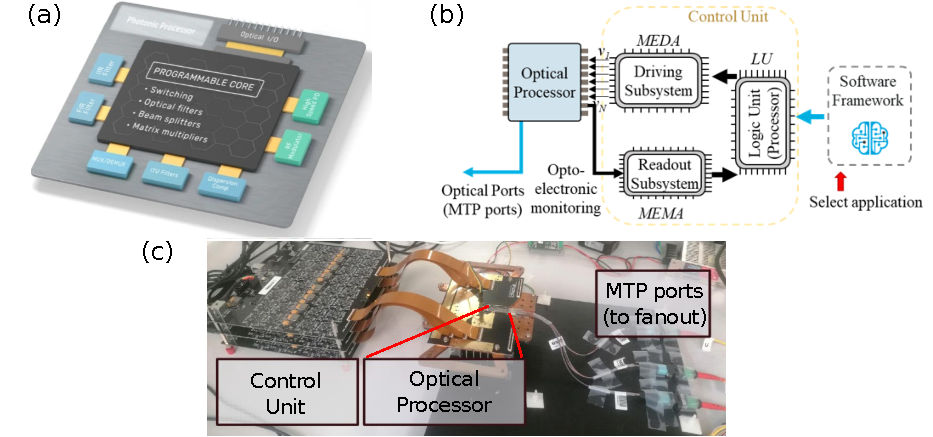
\includegraphics{figures/ch2-smart-subsystems.pdf}
	\end{center}
	\caption{(a) Optical layer of the processor with the core, I/Os, and high-performance blocks, (b) assembled chip with control unit and access fibers, (c) interconnection diagram between optical system, control unit and software layer.}
	\label{fig:ch2-smart-subsystems}
\end{figure}

Figure~\ref{fig:ch2-smart-subsystems} provides a glance of what is inside the first-generation Smartlight case.
In Fig.~\ref{fig:ch2-smart-subsystems}(a) we observe a diagram with the main block components of the reconfigurable photonic integrated circuit (PIC) with a core (dark gray) containing the reconfigurable PUC mesh which is connected through waveguides to high-performance blocks (HPBs).
The blue HPBs are pure optical circuits such as filters and multiplexers.
The green HPBs are RF optoelectronic components that enable microwave photonic applications.
All these subsystems enable the PIC to implement a wide range of applications such as filtering, splitting, switching, among others that will be covered in the next chapter.
Optical inputs/outputs (I/O) ports allow to-be-processed signals to flow in and out of the unit once the operation has been performed.
The chip is connected optically through a fiber array with 64 ports (see Fig.~\ref{fig:ch2-smart-subsystems}(c)), from which 28 are routed to the mesh core and serve as I/O ports while the rest are kept for internal testing.
These 64 PIC ports are distributed among the three MTP connectors at the front panel.
Additionally, the chip has been packaged electronically through wire bonding interconnection to a printed circuit board (PCB).
On the electronic layer, 304 on-chip phase actuators are controlled by a board-integrated programmable multichannel electronic driving array (MEDA) source connected to the logic unit (LU) (Fig.~\ref{fig:ch2-smart-subsystems}(c)).
Similarly, 40 on-chip photodetectors are measured through an on-board readout system connected to the logic unit.
This monitoring system is the so-called multichannel electronic monitoring array (MEMA) that provides feedback on the optical power at each mesh port and four HPBs (Fig.~\ref{fig:ch2-smart-subsystems}(c)).
Closing the workflow, the software running in the LU actuates over the photonic system and can get instant data of the circuit configuration.
The overall operation (set and readout times) is dominated by the driving unit, setting the reconfiguration time of the system to 15–90 ms.

\begin{figure}[h]
	\begin{center}
		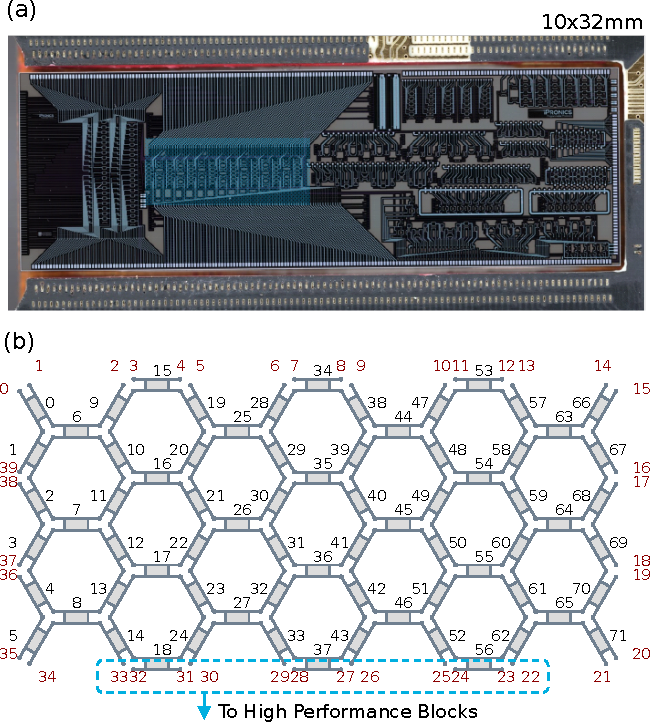
\includegraphics{figures/ch2-sw-smart-mesh.pdf}
	\end{center}
	\caption{(a) Picture of the chip with the highlighted region of the reconfigurable core, (b) schematic of the waveguide mesh core \cite{perez-lopez_general-purpose_2024}.}
	\label{fig:ch2-smart-mesh}
\end{figure}

The photonic stage is integrated into a silicon-on-insulator chip that includes a reconfigurable core of 72 Programmable Unit Cells (PUC) distributed in a flatted hexagonal mesh topology (see Figure~\ref{fig:ch2-smart-mesh}(a)) \cite{perez-lopez_general-purpose_2024}.
At the optical layer, the chip is optimized for C-band operation.
As described in Figure~\ref{fig:ch2-smart-mesh}(b), the mesh core has 40 output ports, 12 connected to on-chip HPBs (2 lattice filters of order 4, 1 coupled-ring filter, and 1 Ring-assisted MZI filter of order 4).
Further study and developments related to the HPBs lies beyond the scope of this thesis.
As described Sec.~\ref{sub:the_mach-zehnder-interferometer}, each PUC consists of a Mach-Zehnder Interferometer (MZI) with two thermo-optic phase actuators.
By tuning one of the arms, the user can modify the coupling factor of the 2-by-2 block.
For independent coupling factor and phase response configuration, the user/system can configure both arms.
The insertion loss and efficiency have been characterized across many chips and two wafers, resulting in 0.48 dB/PUC and 1.3 mW/π, respectively.
The basic unit length (BUL), i.e., the length of a PUC, and the basic unit delay (BUD), i.e., the signal delay during propagation through a PUC, are also characterized as 811 um and 11.25 ps, respectively.
Propagation losses are measured between 1.5 and 2.5 dB/cm for different waveguide widths and dies.
Finally, fiber-chip coupling loss ranges between 1.5 dB to 3 dB, for different coupling techniques.
For the scope of this paper, we employed a device with 3 dB loss per facet.
For further information, a detailed explanation of all the photonic specifications of first-generation Smartlight is provided in Table~\ref{tab:ch2-phot_specs}.

% \begin{noindent}
\begin{table}[ht!]
  \small
	\centering
	\begin{tabular}{|m{4cm}|m{1.0cm}|m{1.0cm}|m{1.0cm}|m{1.5cm}|m{5.5cm}|}
		\hline
		\multirow{2}{*}{\textbf{Specification}}         & \multicolumn{3}{c|}{\textbf{Value}} & \multirow{2}{*}{\textbf{Units}} & \multirow{2}{*}{\textbf{Description}}                                                                                                                                                                                                                                                                                                                              \\
		\cline{2-4}  % Line only below column 2 
		           & Min     & Typ.     & Max  &   &
		\\
		\hline
    Number of PUCs   &    & 72    &      & PUCs   & Arranged in the hexagonal lattice as shown in Figure~\ref{fig:ch2-smart-mesh}
		\\
		\hline
		Fiber to chip coupling loss/facet & 1.8  & <3.34 & 3.6  & dB & Fiber to chip coupling loss.
    \\
		\hline
		On-chip routing losses from and to optical I/Os & 5 & <7 & 8.4 & dB & On-chip routing losses from waveguides going into the mesh and coming out from it. 
    Facet loss not included.
		Mesh loss not included.
		\\
		\hline
		Losses per PUC  & 0.46  & 0.50  & 0.55  & dB   & 
    \\
		\hline
		Extinction ratio of PUCs & 32 & 35  & 44  & dB  & Difference between the maximum and minimum optical power obtained by sweeping a PUC's phase shifter. 
    Through port: 33 dB (Typ), Cross port: 44 dB (Typ).
		\\
		\hline
		30-dB isolation bandwidth of PUC & 30 & 45 & 65 & nm & Cross port: >60 (Median), Through port: 45 dB (Median).
		\\
		\hline
		±2\% Uniformity bandwidth & 3 & 5.5 & 15 & nm & Characterized for a coupling factor configuration of 50\%.
		Cross port: 8.1 ± 4.5 nm, Through port: 5.1 ± 1.55 nm.
		\\
		\hline
		Power consumption per phase shifter & 1.2 & 1.34 & 2.0 & mW/π  & 
		\\
		\hline
		Single-channel reconfiguration speed & & <14 &  & ms & <62.5 ms for 160 channels (writing).
		<0.3 ms for 50 channels (reading). 
    \\
		\hline
    Basic unit length (BUL) & & 811.41 &  & µm   & Length of a PUC. It sets the spatial resolution of the circuits programmed within the mes.
    \\
		\hline
    Basic unit delay (BUD) & & 11.25 &  & ps & Access path to the mesh accumulates 48 ps additionally.
		\\
		\hline
	\end{tabular}
  \caption{Optical specifications of a first-generation Smartlight unit.}
  \label{tab:ch2-phot_specs}
\end{table}
% \end{noindent}

% subsection  Optical Specifications (end)

% section Smartlight: The Field Programmable Photonic Gate Array (end)
\section{Software stack}\label{sec:software_stack}

\begin{figure}[h]
	\begin{center}
		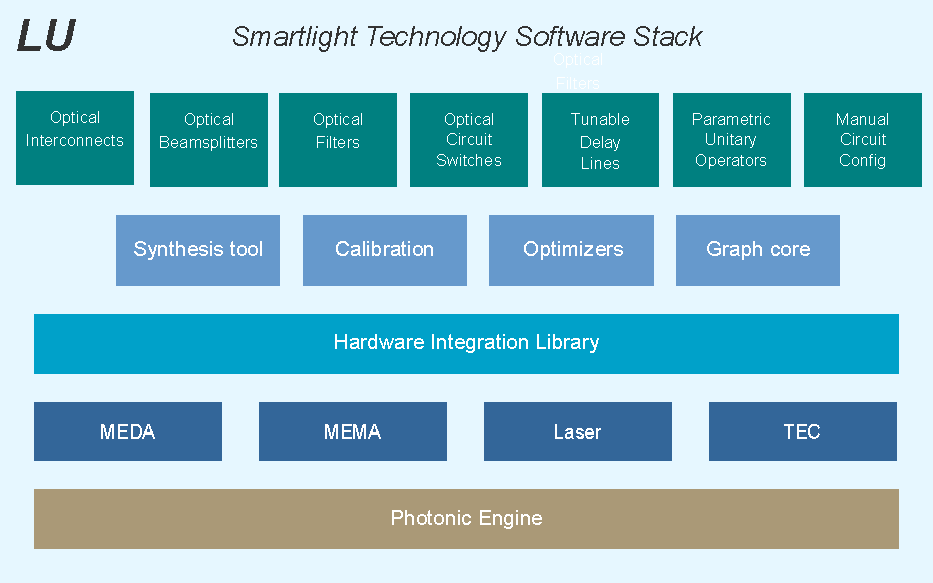
\includegraphics{figures/ch2-sw-stack.pdf}
	\end{center}
	\caption{Software stack developed under the framework of this thesis to control and operate on the reconfigurable PIC.}\label{fig:ch2-sw-stack}
\end{figure}

Programmable photonics involves a software framework that encompasses a wide array of algorithms, methods, or routines executed by a logic unit (LU) running a GNU/Linux distribution.
These serve primarily to configure specific functionalities within a Photonic Integrated Circuit (PIC) and to optimize the backplane.
These routines can be categorized based on their intended outcomes or their specific requirements as shown in Figure~\ref{fig:ch2-sw-stack}.
The first layer includes the low-level functions necessary to maintain the chip's temperature stable (TEC), drive (MEDA) and read (MEMA) from the photonic and electro-optic components, and control the tunable laser to feed signals into the system.
These subsystems of Smartlight are coordinated through the hardware integration layer that handles the calls to them and orchestrates the submodule communication.
On top of this layer sits a group of fundamental routines dedicated to enable high-level user functionalities and ensure the system's operation at an optimal point.
Among these we have PIC calibration routines (refer to Sec.~\ref{sub:calibration}), a set of finely tuned optimizers, a graph model of the PIC (see Sec.~\ref{sub:graph_layer}) and an elaborate synthesis tool that maps user configurations into low-level parameters to drive the photonic engine.
These modules often rely on calls to each other to yield observable outputs.
For instance, optimizer routines power the calibration of the electro-optical response of each phase shifter within the circuit, eliminating the need to integrate optical monitors into the waveguide mesh.
Additionally, these routines can extract valuable information such as the power consumption of individual units, accumulated losses to identify and record defects within the circuit.
The data collected can then be fed into a graph model to leverage on well-known network optimization algorithms, e.g., Dijkstra or A*, to optimize both the circuit's functionality and resource utilization.
The specific technical details of these software libraries will be presented in Chapter~\ref{chap:applications_using_fppgas}.
The same outcomes from the optimization, calibration and graph core utilities enable the manual and automatic synthesis of circuits in the first-generation Smartlight mesh.
The final layer exposes a Python API to the end users via the \lstinline|Smartlight| class which exposes the functionalities in Figure~\ref{fig:ch2-sw-calib} top layer.
This layer also includes a set of virtual scopes to monitor the status of the mesh configuration, the on-chip photodetector readings and a spectrum analyzer tool.
Examples of how to use these high-level methods and the monitors are presented in detail in Chapter~\ref{chap:applications_using_fppgas}.

\begin{figure}[h!]
	\begin{center}
		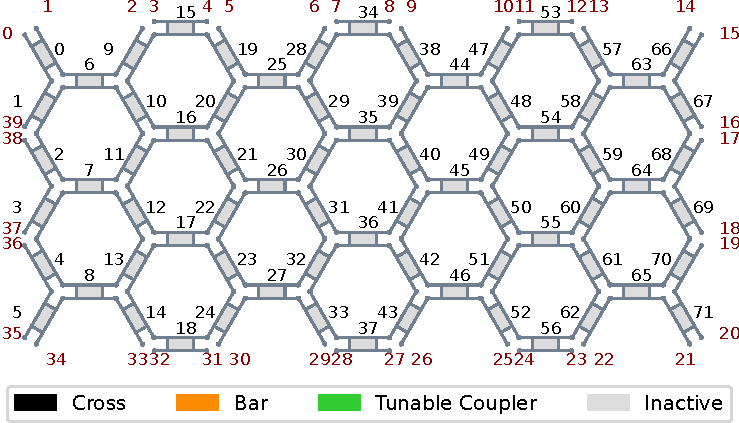
\includegraphics{figures/ch2-sw-mesh.pdf}
	\end{center}
	\caption{Representation of the first-generation Smartlight PIC hexagonal mesh developed during this thesis to monitor and track the status of the PUCs on demand.}\label{fig:ch2-sw-mesh}
\end{figure}

The latest Python API developed during this thesis is the \lstinline|iPronics_smartlight_v.1.12.1| which is compatible with Linux, macOS and Windows machines.
The software is tailored to work with the hexagonal mesh array presented in Section~\ref{sec:smartlight_fppga} of the iPronics first-generation Smartlight solution.
Although the higher layers in Figure~\ref{fig:ch2-sw-stack} are architecture agnostic, the lower levels are not.
The hardware integration layer has been developed to work with the MEDA, MEMA, TEC and laser subsystems inside Smartlight.
Nevertheless, the software infrastructure has been laid out in such a way that the inclusion of new peripherals (i.e., to favor version upgrades) can be performed without particular overheads.
Figure~\ref{fig:ch2-sw-mesh} depicts the output from the \lstinline|Core_Monitor| visualizer created to monitor the current status of the Smartlight photonic core.
Each PUC is represented as a rectangle with four ports (2 inputs and 2 outputs).
The label of each PUC is shown in black and the optical ports in red.
This monitor queries the MEDA registers to collect information about active PUCs in the system and plots it to the user using a color code system.
PUCs configured in cross, bar, coupler and inactive states are painted black, orange, green and gray, respectively.
Since this scope is showing the status of a mesh that has not been programmed, all PUCs are painted gray (i.e., inactive) which means that no control signal has been applied to their phase shifters which renders them at a random fabrication state.

\subsection{Calibration}\label{sub:calibration} % (fold)

\begin{figure}[h]
	\begin{center}
		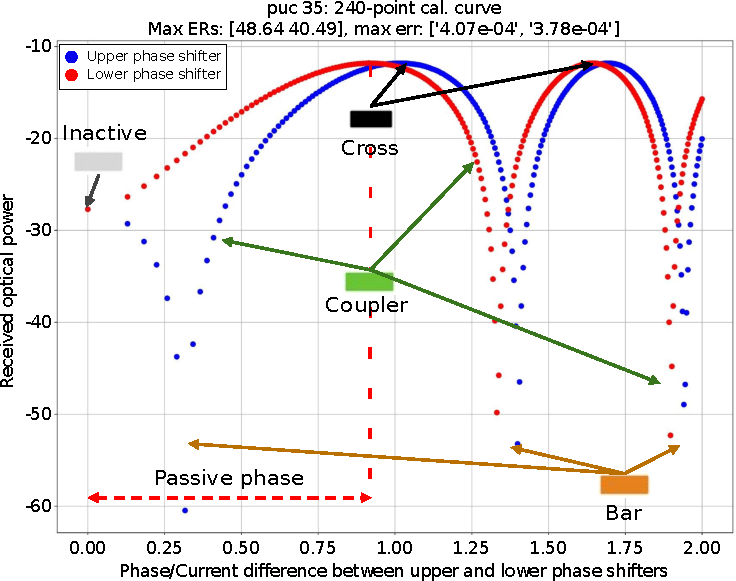
\includegraphics{figures/ch2-sw-calib.pdf}
	\end{center}
	\caption{Calibration trace of a PUC.
		Black/orange/green arrows point to the currents that set the cross/bar/coupler state of a PUC.
		These traces are essential to estimate the manufacturing passive phase of a PUC.
	}\label{fig:ch2-sw-calib}
\end{figure}

To program the Smartlight mesh effectively all PUCs must be calibrated previously, meaning that the electro-optic response of each phase shifter has been characterized and modelled correctly.
The calibration algorithm of a hexagonal mesh is an iterative process that relies on driving the phase actuators of the PUCs that form a path in the mesh until a set of currents that maximize the path's power has been found.
This set of currents corresponds to the biases needed to set these PUCs to cross and bar state, depending on the path of interest.
Once these points have been well-defined and set, the currents driving one PUC's phase shifters within the path can be swept to obtain their calibration traces as shown in Figure~\ref{fig:ch2-sw-calib}.
The calibration curves of a PUC's phase shifters provide details on the relationship between the applied current and the actual phase set by the actuator.
Fig.~\ref{fig:ch2-sw-calib} shows that, although the actuators should be at cross state by default (refer to Sec.~\ref{sub:the_mach-zehnder-interferometer}), they start at an intermediate point between bar and cross due to manufacturing errors.
The phase difference between the ideal cross state and the initial state is the so-called \textbf{passive phase}.
Since in this case the power is measured at the PUC's cross port, the maxima in these traces correspond to different cross-state currents in the 2\(\pi\) cycles.
Likewise, the minima correspond to the currents that set circuit to bar-state.
All the other currents between these previous points correspond to intermediate states that set the PUC as a tunable coupler (i.e., \(0 < k < 1\)).
The calibration routine of the first-generation Smartlight system allows setting \lstinline|k| values with a 0.001 resolution.
As presented in Eq.~\eqref{eq:ch2-phase_current}, the relationship between phase and driving current is non-linear, thus explaining why the cross and bar periods in Fig.~\ref{fig:ch2-sw-calib} get shorter for higher currents.

\begin{equation}
	\begin{aligned}
		\phi_{\text{up}} & = \rho_{2\_\text{up}} \cdot I^2 + \rho_{3\_\text{up}} \cdot I^3 + \alpha \\
		\phi_{\text{lo}} & = \rho_{2\_\text{lo}} \cdot I^2 + \rho_{3\_\text{lo}} \cdot I^3,
	\end{aligned}
	\label{eq:ch2-phase_current}
\end{equation}

where \(\phi\) corresponds to the phase applied by the actuator, \(\alpha\) is the passive phase and \(\rho_2\), \(\rho_3\) are the quadratic and cubic current-phase factors.
The last three parameters are the ones that must be identified for all phase actuators for the correct programming of circuits on the Smartlight mesh.
The full calibration routine involves creating several paths within the mesh, each with more PUCs than the previous one, so that over a number of iterations the calibration parameters of all phase actuators have been collected.
Further details about the calibration process can be found in \cite{lopez-hernandez_automatic_2022,jia_calibration_2024}.

% subsection Calibration (end)
\subsection{Circuit synthesis}\label{sub:circuit_synthesis} % (fold)

\begin{lstlisting}[caption={Manual synthesis of a basic circuit using the first-generation Smartlight API}, label=lst:ch2-sw-synthesis]
from smartlight import Smartlight
from smartlight.graphics import (
    CoreMonitor,
    MEMAMonitor,
    OpticalResponseVisualizer,
)
# Instantiate system
smart = Smartlight()
smart.set_input_port(0)
# Define circuit configuration
basic_circuit = [ (0, "x"), (6, "x"), (10, "x"), (16, "="), (20, "="), (19, "x") ]
smart.manual_circuit_configuration(basic_circuit)
# Monitor waveguide mesh
core_monitor = CoreMonitor(smart)
core_monitor.plot_mesh_status()
# Turn on laser
smart.enable_laser()
# Monitor on-chip PDs
mema_monitor = MEMAMonitor(smart)
mema_monitor.plot_current_mema_status()
\end{lstlisting}

The process to implement a basic circuit on the first-generation Smartlight mesh using the Python package developed during this thesis is exemplified in Listing~\ref{lst:ch2-sw-synthesis}.
The first step is to import the main libraries that enable user-device interaction.
\lstinline|Smartlight| represents the class that, once instantiated, boots Smartlight along all its subsystems.
\lstinline|CoreMonitor| is a virtual scope that monitors and tracks the PUC status in the mesh to enable circuit visualization (refer to Figure~\ref{fig:ch2-sw-mesh}).
\lstinline|MEMAMonitor| provides a power visualizer of on-chip photodetector readings (see Figure~\ref{fig:ch2-sw-synthesis}(b)).
\lstinline|OpticalResponseVisualizer| performs a laser sweep to capture the transmission spectral response of circuits configured on the mesh such as the ones in Section~\ref{sec:filters}.
Once the system has booted up, circuits can be implemented on it using the \lstinline|manual_circuit_configuration()| instruction which accepts a \lstinline|List(Tuple(puc_id, state))| to configure the mesh.
Where \lstinline|puc_id| corresponds to the PUC label as depicted in Figure~\ref{fig:ch2-sw-mesh} and \lstinline|state| can either be \lstinline|"x"| for cross, \lstinline|"="| for bar and \lstinline|k| (a floating-point number) for tunable coupler.

In Figure~\ref{fig:ch2-sw-synthesis} we observe the result of running Listing~\ref{lst:ch2-sw-synthesis} on a first-generation Smartlight system.
Figure~\ref{fig:ch2-sw-synthesis}(a) shows the \lstinline|CoreMonitor| output where we observe that all PUCs have been configured correctly to establish an optical path between ports 0 and 5.
Figure~\ref{fig:ch2-sw-synthesis}(b) contains the \lstinline|MEMAMonitor| output for this circuit which, as expected, has routed most of the optical power from input 0 to the photodetector connected to port 5.

\begin{figure}[h]
	\begin{center}
		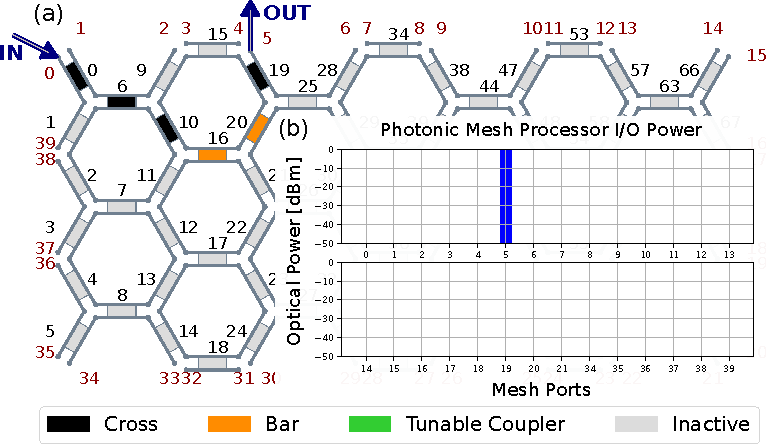
\includegraphics{figures/ch2-sw-synthesis.pdf}
	\end{center}
	\caption{Basic interconnect circuit synthesized using manual configuration.
		Individual PUC states are defined using 'x', '=' or 'k' states.
	}\label{fig:ch2-sw-synthesis}
\end{figure}

An additional method to configure circuits on the mesh is \lstinline|set_coupling_factor_phase()| which allows setting not only the coupling factor \(k\) but also the cross-phase \(\Delta\) (refer to Section~\ref{sub:the_mach-zehnder-interferometer}) of each individual PUC.
The \lstinline|set_coupling_factor_phase()| accepts as arguments a \lstinline|List(Tuple(puc_id, List(state, cross_phase)))| where \lstinline|cross_phase| corresponds to the PUC's common transmission phase in radians, and the rest of parameters remain the same as described above.
This functionality provides the end-user with very precise control over the amplitude and phase of the synthesized circuits.
Practical examples of how this instruction can be the key enabler of certain phase-sensitive applications are presented in Chapter~\ref{chap:applications_using_fppgas}.

% subsection Circuit synthesis (end)
\subsection{Graph layer}\label{sub:graph_layer}

To control the photonic processor, a software layer based on graphs is used.
Graph theory \cite{kerchove_automated_2023} provides a framework for analyzing and solving problems related to connectivity, paths, cycles, and other properties of graphs.
A graph model representing the mesh in the first-generation Smartlight system has been developed and is integrated with the product.
In the latter, all the connectivity and topology of hexagonal mesh can be abstracted into a model, in which the optical ports of the PUCs are represented as nodes in the graph, and the flow of light in the waveguides can then be represented by edges connecting these nodes.
One challenge in graph representation of hexagonal mesh is the feedback loops in the circuit.
To address this, we chose the directed graph with eight artificial nodes \cite{chen_graph_2020} for our model, where each port of PUC is represented with two artificial nodes, for inbound and outbound of the signal.
Specific details of the graph implementation are provided in reference \cite{xie_software-defined_2024}.
The PUC phase shifters are modeled by arcs with the direction of input and output ports.
The graph representation incorporates performance metrics for each connection, which means each arc is assigned a weight as expressed by Equation~\eqref{eq:ch2-graph_weight} where IL is the PUC insertion loss, BUL is the PUC basic unit length, and P is the PUC's power consumption.

\begin{equation}
	w = c_1 \cdot \textit{IL} + c_2 \cdot \textit{BUL} + c_3 \cdot P + \dots
	\label{eq:ch2-graph_weight}
\end{equation}

Hence, the weight can be calculated according to these figures of merit (FOM) by only changing the distribution of weights \(c_i\) \cite{lopez_auto-routing_2020}.
The underlying graph layer in the Smartlight API is one of its most powerful libraries as it powers several applications and allows defining circuit implementations that optimize insertion losses, power consumption and other non-ideal effects automatically.
The auto-routing algorithm powered by this graph model assumes a critical role in this process, as it automatically determines optical paths and interferometric structures within the waveguide mesh topology.
Furthermore, the latter routine introduces groundbreaking self-healing and fault-tolerant capabilities for the PIC.
When confronted with damaged areas within the mesh, the algorithm is adept at identifying alternative suboptimal paths to be used by circuits.

% subsection Graph layer (end)
\subsection{Automatic synthesis}\label{sub:automatic_synthesis} % (fold)

\begin{lstlisting}[caption={Automatic synthesis of a basic circuit using the first-generation Smartlight API}, label=lst:ch2-sw-auto-synthesis]
	# Automatic configuration
	PUCs_configuration = smart.interconnect_auto(input_port=0, output_port=6)
	\end{lstlisting}

Automatic synthesis involves selecting and arranging PUCs in a manner that automatically defines the paths taken by the optical signal fed into the chip.
For a given specification, such as achieving a 10 ns delay between two specific optical ports, multiple solutions may exist.
In this context, a software layer powered by a graph model is capable of determining the configuration solutions that minimize the number of PUCs required, the driving power, etc. depending on the FOM to optimize by the solution of interest.
With a graph model at hand we can leverage on ubiquitous, yet extremely influential, algorithms such as Dijkstra/A* \cite{bierlaire_optimization_2015} and network optimizers to facilitate the convergence on optimal circuit configurations, as evidenced by references \cite{lopez_auto-routing_2020,perez-lopez_multipurpose_2020}.
The resultant configurations can be stored for future use and employed to dynamically configure the circuit.
Listing~\ref{lst:ch2-sw-auto-synthesis} shows the example of how to implement the interconnect circuit defined in Listing~\ref{lst:ch2-sw-synthesis} using an automatic instruction based on the graph layer presented previously.
Note that now there's no need to define the individual states of the PUCs as they are returned and configured by the \lstinline{interconnect_auto} instruction.
In this particular case the resulting mesh configuration is the same one presented in Figure~\ref{fig:ch2-sw-synthesis}.
An extensive set of examples of how to perform automatic synthesis of several applications and their implementation details are presented in Chapters~\ref{chap:applications_using_fppgas} and \ref{chap:universal_unitary_operators}.

% subsection Automatic synthesis (end)
% section Software stack (end)

